93. $\cfrac{3}{5x-1}+\cfrac{4}{3x+1}\geqslant1\Leftrightarrow\cfrac{9x+3+20x-4-15x^2-5x+3x+1}{(5x-1)(3x+1)}\geqslant 0\Leftrightarrow
\cfrac{3x(9-5x)}{(5x-1)(3x+1)}\geqslant 0.$ Применив метод интервалов, найдём ответ:
\begin{figure}[ht!]
\center{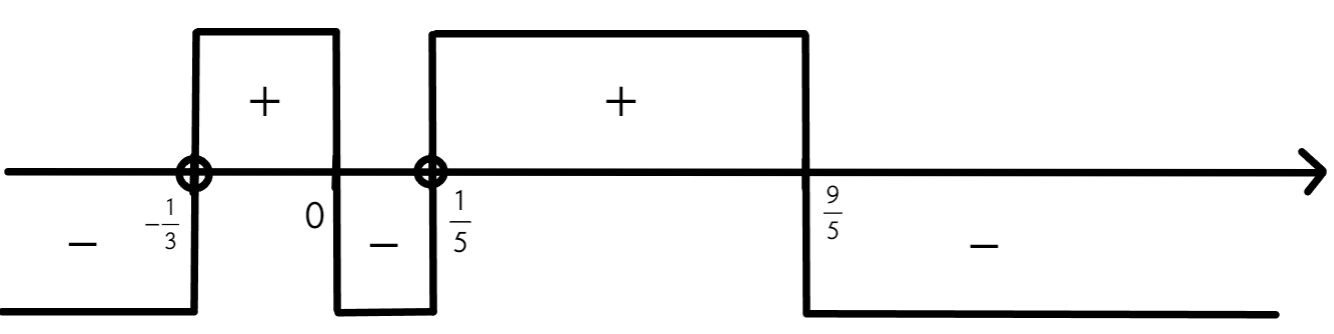
\includegraphics[scale=0.35]{int93.png}}
\end{figure}
$x\in\left(-\cfrac{1}{3};0\right]\cup\left(\cfrac{1}{5};\cfrac{9}{5}\right].$\newpage\noindent
